\chapter{Overlap Add Reconstruction of Voiced Speech} \label{chap:overlapAdd}

In this next chapter, we will describe and discuss the proposed system architecture for the overlap add reconstruction of voiced speech. Besides that, both the whisper activity detection and speech segmentation algorithms that are used in the proposed system for silence detection and Voiced/Unvoiced decisions are introduced and discussed.

The system is meant to take in whispered speech as input, and output a reconstructed voiced speech signal, by first utilizing the LPC filtering mechanism presented in Chapter \ref{chap:filt}, and exciting that with both synthetic pulses, for the case of voiced speech segments and noise in the case of unvoiced regions. 

\section{Proposed System Architecture}

The diagram for the complete system architecture can be seen in Figure \ref{fig:systemDiagram}. It works by first taking in input frames which are 512 samples long, and then applying a 50\% overlap to these frames, along with the previous frame in order to obtain a 1024 sample windowed frame. Then the PSD of this frame is computed through the ODFT, as shown in the previous chapter, which gets mixed with PSD that was obtained in the previous frame. This is done in order to obtain a smooth transition between filters across frames. This mechanism can be visualized in Figure \ref{fig:pulseMap}, where according to the relative position of each pulse within the current frame $\alpha_k$, a new filter is created by mixing the current frame's PSD with the one obtained in the previous frame. This is done by means of a linear interpolation between the two PSDs, as shown in Equation (\ref{eq:psdInterpolation}).

\begin{equation}
    PSD_{pulse}[k] = (1-\alpha_k) PSD_{j-1}[k] + \alpha_k PSD_j[k]
    \label{eq:psdInterpolation}
\end{equation}

From this new PSD, and using the same LPC analysis mechanism as in the previous chapter, a new filter $H_j[k]$ is obtained, that is only used for the pulse in question. This newly generated filter is then used to filter the pulse in the time domain, and the result is then added to the output at \texttt{mainBuff[n]}, using the same overlap logic that was used in Chapter \ref{chap:pulseGen} for the pulse generation and concatenation. 

For mixing the PSDs of the current and previous frames, the mixing factor $\alpha_k$ is defined as shown in Equation (\ref{eq:alphaDef}), where $lastPulsePos$ is the current sample number and $N_2$ is the total number of samples in the frame.

\begin{equation}
    \alpha_k = \frac{\text{lastPulsePos}}{N_2}
    \label{eq:alphaDef}
\end{equation}

Before computing the filter, tilt compensation is applied to the PSD, as per the method described in the previous chapter. This tilt factor is precomputed beforehand at startup and is applied equally to all interpolated PSDs, as the changes in the generated pulse frequencies are not significant enough to warrant a per-pulse tilt compensation. 

\begin{figure}[H]
    \centering
    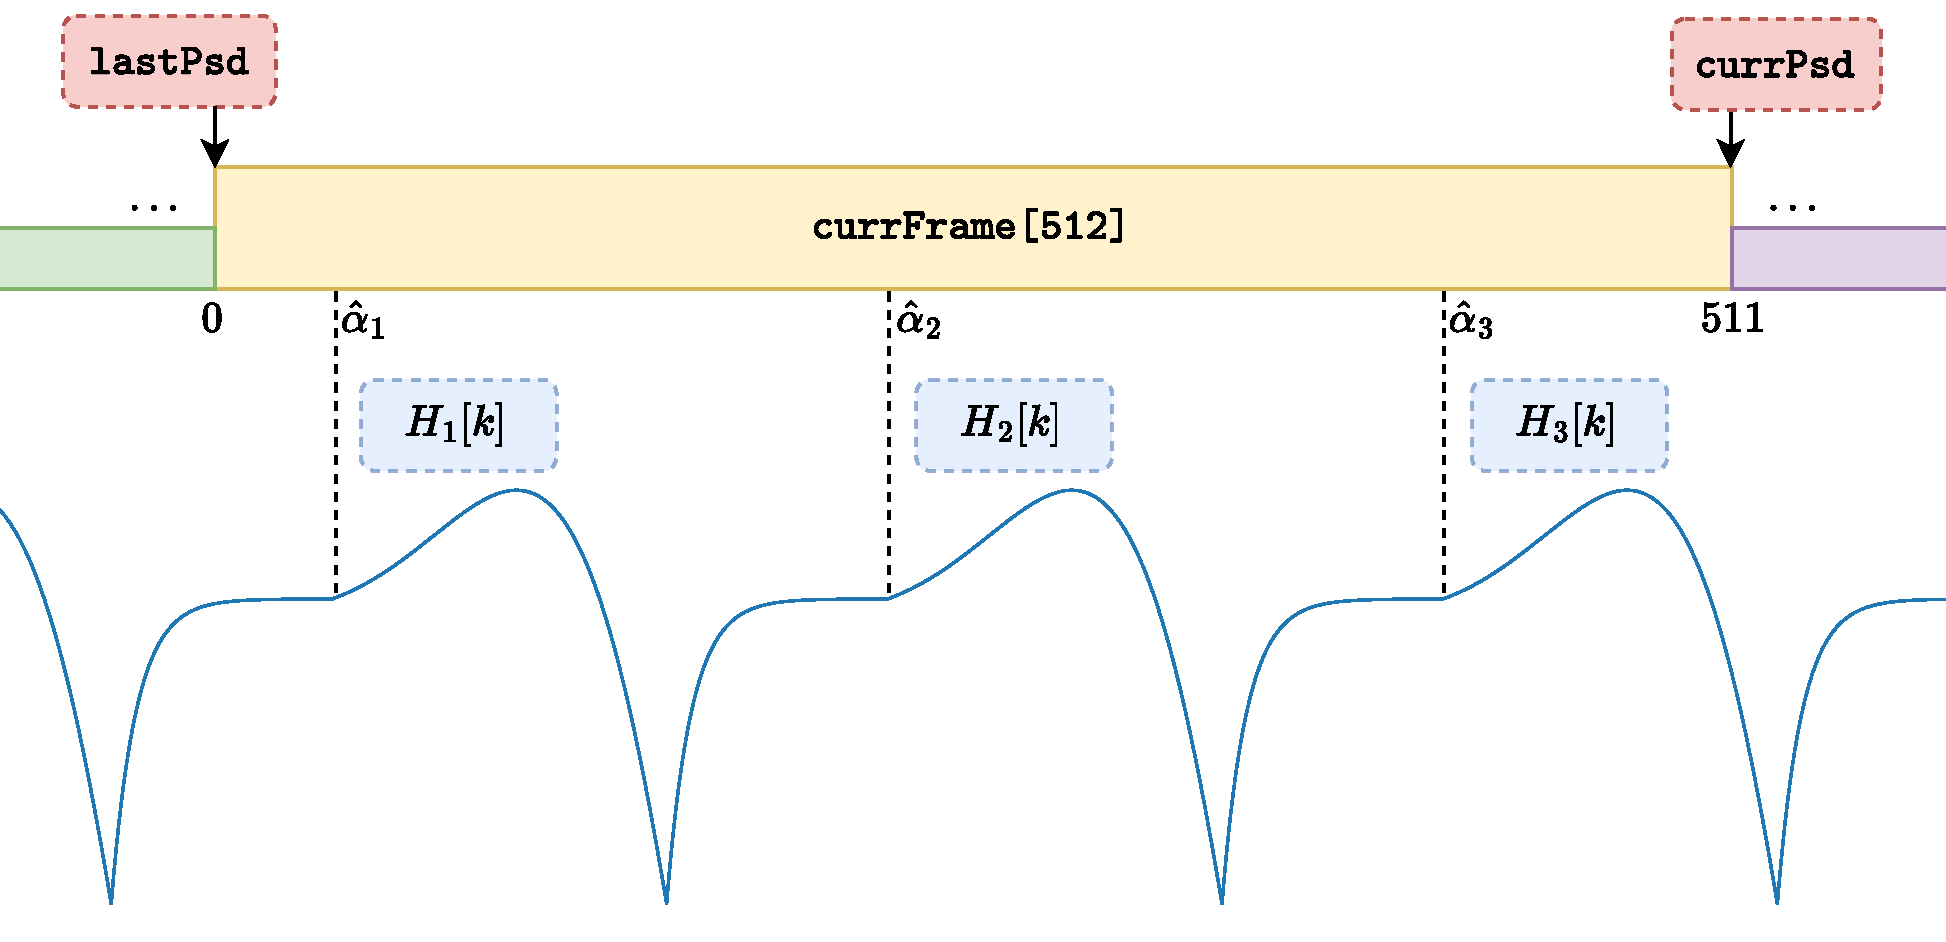
\includegraphics[width=0.9\textwidth]{chapter6/pulseMap.pdf}
    \caption{Individual pulse filtering mechanism}
    \label{fig:pulseMap}
\end{figure}

The system also includes a mechanism for whispered activity detection and another for speech segmentation, which are used to determine the activity of the signal and how to treat each frame in terms of whether it is voiced or unvoiced. These two mechanisms are also used to determine the fundamental frequency of the voiced segments of the signal, by triggering the $f_0(t)$ contour to be applied to the voiced segments of the signal. This contour is also reset whenever there are either silent or unvoiced speech segments. Hopefully this approach improves the prosody of the synthesized speech.

In order to mix both the LF pulse and noise excitation sources in the time domain, a $\beta$ factor is used to determine the relative gain of each source. This factor is determined by the mapping of the centre of gravity to a value between 0 and 1, as we will show in the next sections.

\begin{figure}[H]
    \centering
    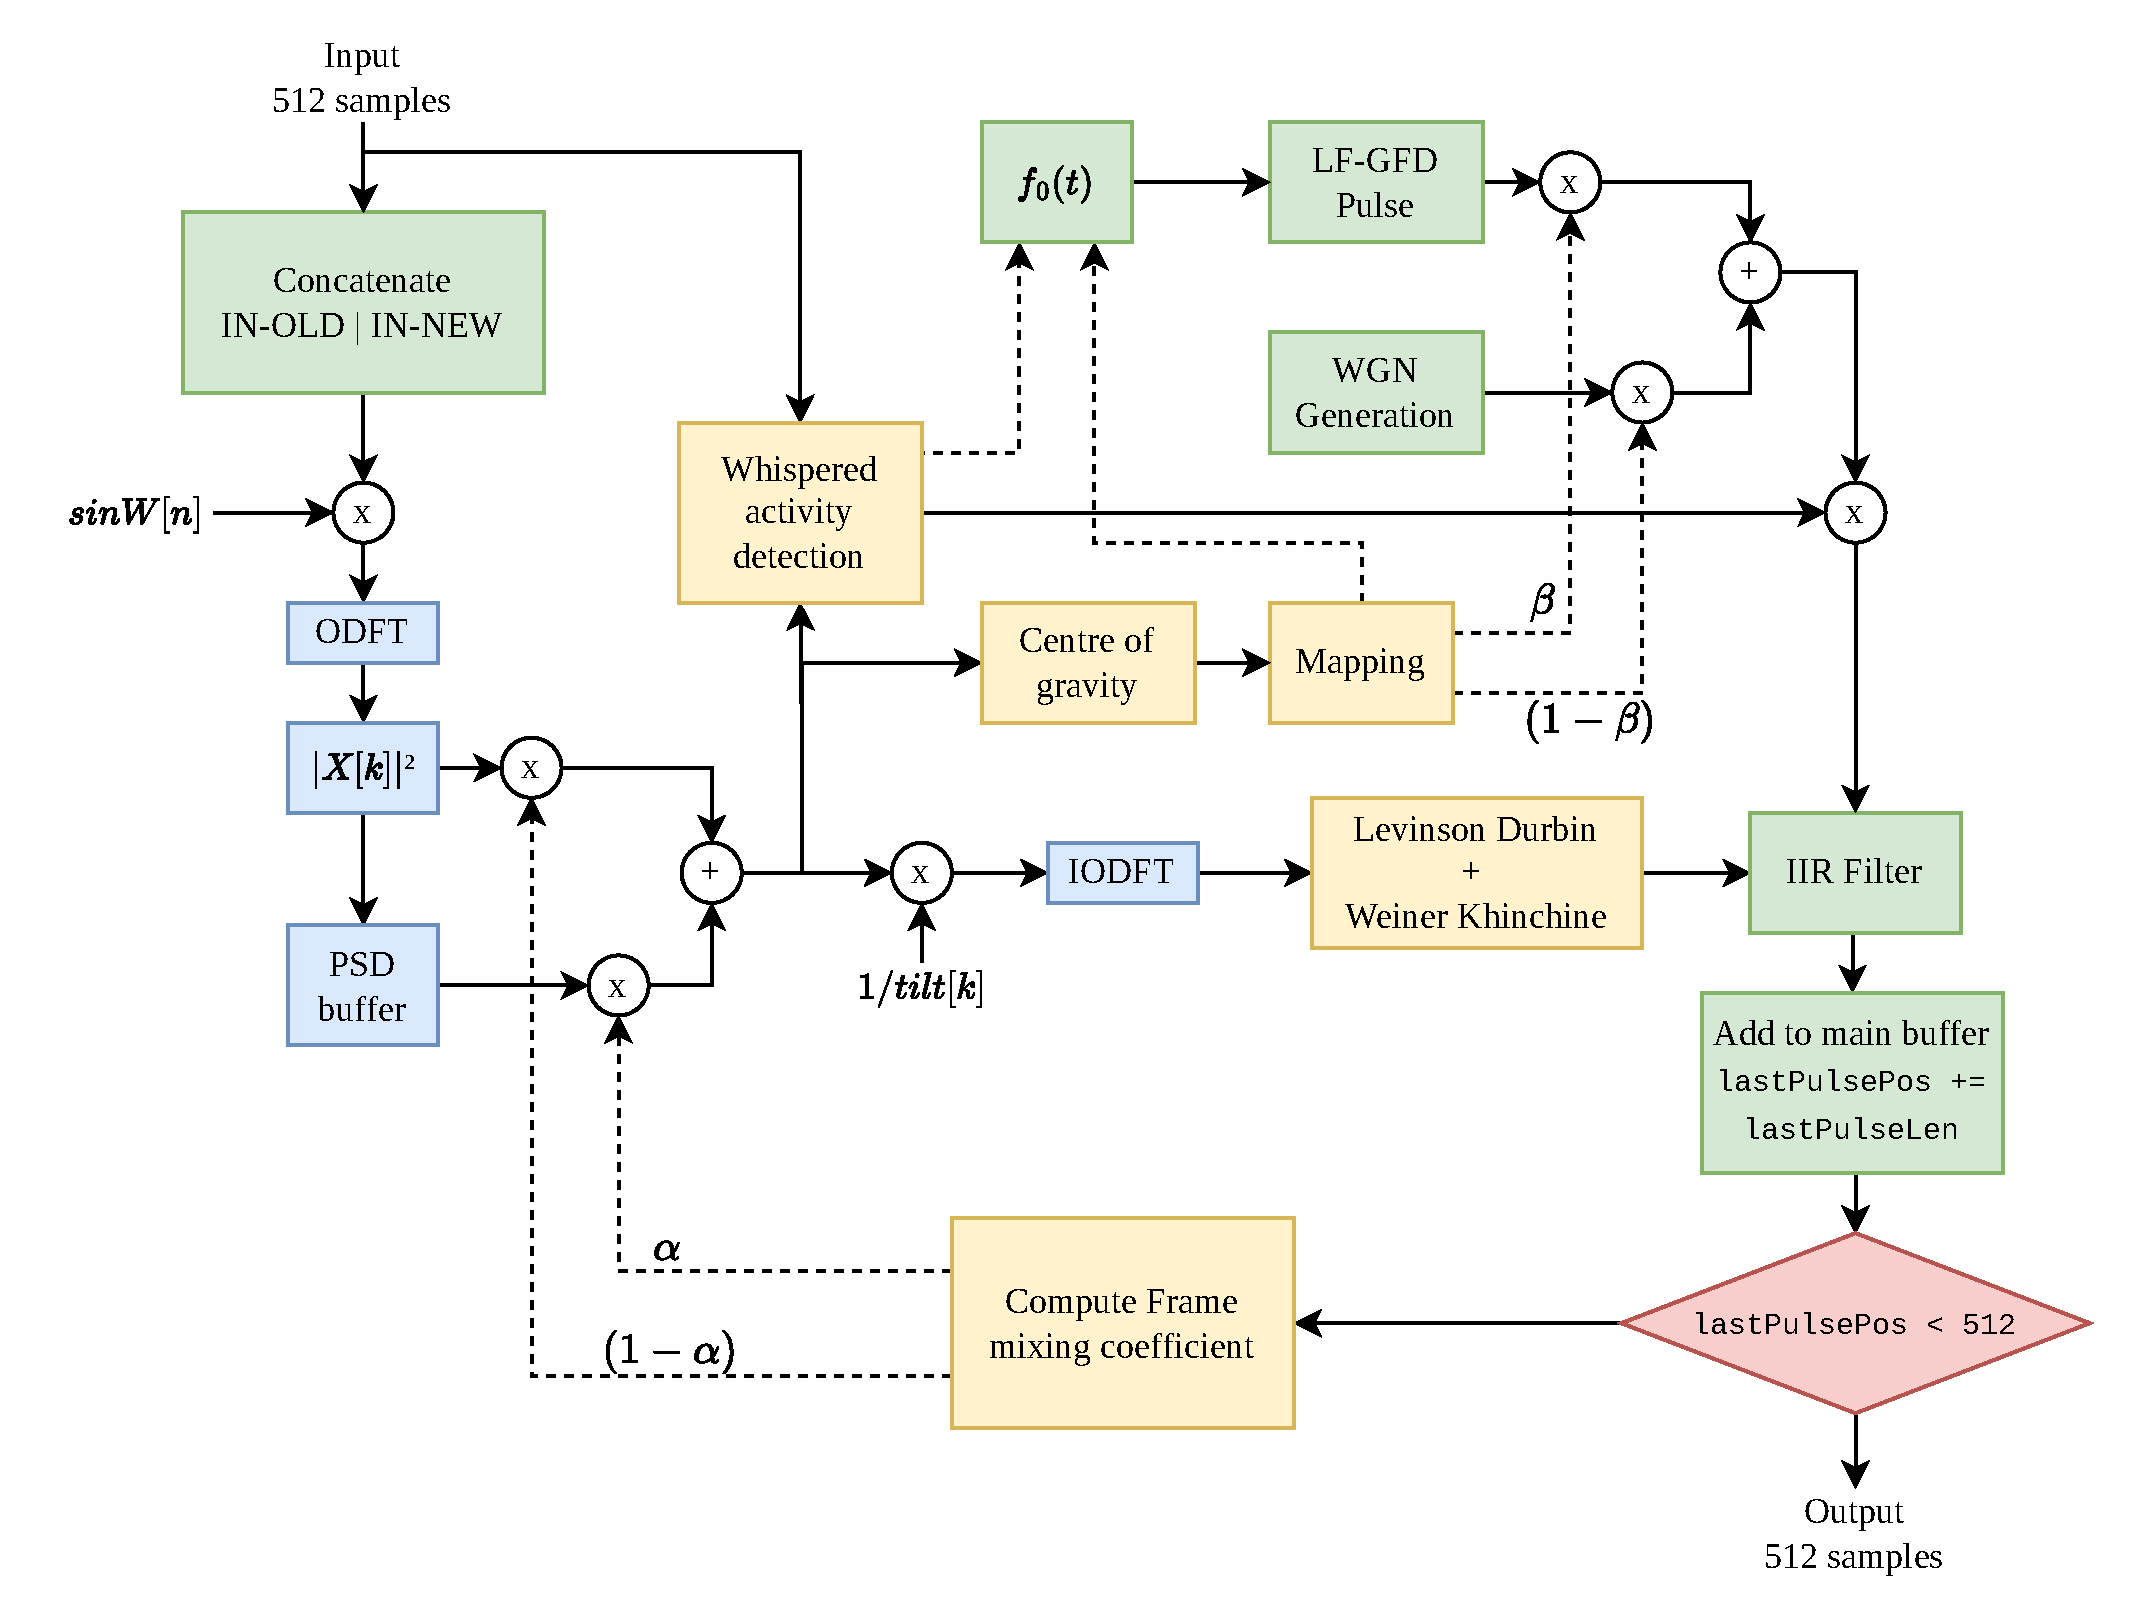
\includegraphics[width=1.0\textwidth]{chapter6/systemDiagram.pdf}
    \caption{Complete System Diagram}
    \label{fig:systemDiagram}
\end{figure}


\section{Whisper Activity Detection}

Similarly to what as proposed by Sharifzadeh et.al in \cite{sharifzadehReconstructionNormalSounding2010}, a modified version of the G.729 whisper activity detection algorithm, as shown in \cite{beritelliPerformanceEvaluationComparison2002}, was utilized for the detection of actual whispered speech in the input signal. This is of course necessary such that the $F_0$ contour can be properly applied to the voiced segments of the signal and such that the voicing decisions are only done on the segments that have actual speech.

In this case, each speech segment is determined as active or idling, by means of both its energy and its zero crossing rate. Three thresholds $\zeta_1$, $\zeta_2$ and $\zeta_{zcr}$, are used to determine the activity of the signal, and the algorithm is as follows, where the energy for a given frame $x[n]$ is given by $E$ and its zero crossing rate is given by $\gamma$:

\begin{equation}
    \text{Activity} = 
    \begin{cases}
        1.0 & \text{if } E > \zeta_2 \\
        0.0 & \text{if } E < \zeta_1 \\
        \frac{\text{sign}{(\gamma - \zeta_{zcr})} + 1}{2} & \text{otherwise}
    \end{cases}
\end{equation}

In the original paper, it is mentioned that the 3 thresholds are adaptive although no reference is made to the way in which these are adapted. As such, it was established that the thresholds would be set empirically on a speaker-by-speaker basis. The way these were set will be discussed in the next section where the results are taken. Figure \ref{fig:g279detection} shows the whispered activity algorithm in action upon a whispered signal.

\begin{figure}[H]
    \centering
    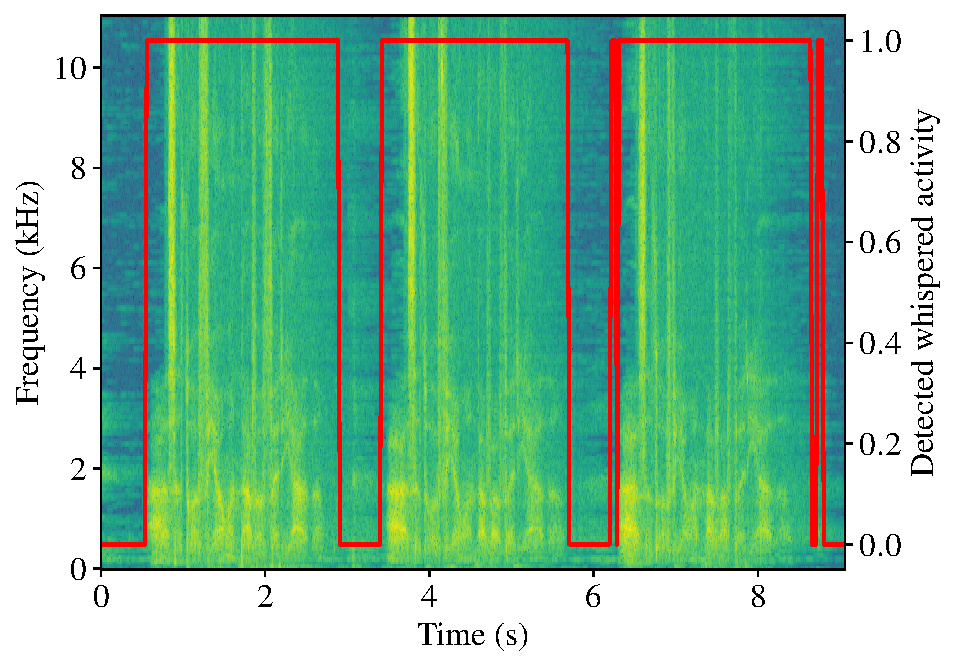
\includegraphics[width=0.8\textwidth]{chapter6/g279detection.pdf}
    \caption{\centering Whispered Detection algorithm applied to a whispered signal - {\it "A asa do avião andava avariada"}}
    \label{fig:g279detection}
\end{figure}

It is worth noting that the previous figure constitutes a best case scenario where all the thresholds are manually set to minimize false activity detection, it is although apparent that the algorithm is not perfect and that there are still some false positives and negatives, particularly when breathing sounds become particularly loud in between whispered utterances. This is to be expected as the algorithm is quite simple and does not take into account the actual content of the signal, only its energy and zero crossing rate.

\section{Speech Segmentation}

As was mentioned in Chapter \ref{chap:sota}, one particular area of research is that of the segmentation or identification of speech segments in whispered speech. This is, determining whether a given segment of whispered speech should be treated as voiced or unvoiced, and if it is voiced, determining the fundamental frequency. 

\subsection{Centre of Gravity}

In the literature review, Chapter \ref{chap:sota}, it has been mentioned that Perrotin et.al. \cite{perrotinGlottalFlowSynthesis2020} identify a simple feature in order to classify each whispered speech into two categories: purely unvoiced sounds, and vocalic unvoiced sounds. Examples of the latter are vowels and voiced consonants. The feature in question is the spectral centre of gravity, otherwise referred to as the spectral centroid \cite{peetersLargeSetAudio2004}, and it is defined as is shown in Equation (\ref{eq:centreOfGravity}), where $S(f)$ is the spectrum of a given whispered speech segment.

\begin{equation}
    \text{Centre of gravity} = \frac{\int_{0}^{Fs/2}f |S(f)|^2 df}{\int_{0}^{Fs/2}|S(f)|^2 df}
    \label{eq:centreOfGravity}
\end{equation}

For the discrete case, we can consider the power spectrum $PSD[k]$ of a given whispered input frame $x[n]$ as the squared magnitude of the ODFT of the frame, and the centre of gravity can be calculated as shown in Equation (\ref{eq:cogDiscrete}), where F[k] is defined as the mean frequency of the k-th frequency bin. This function is effectively the weighted average of the frequency bins of the power spectrum, and can thus provide a good indication of where the energy of the signal is concentrated.

\begin{equation}
    \text{CoG} = \frac{\sum_{0}^{N/2}PSD[k]F[k]}{\sum_{0}^{N/2}PSD[k]}
    \label{eq:cogDiscrete}
\end{equation}

Figure \ref{fig:centreOfGravity} shows how the centre of gravity changes throughout the signal. It is to be noted that the centre of gravity is generally lower for voiced segments of the signal, and higher for unvoiced segments. This is due to the fact that the energy of the signal is concentrated in the lower frequencies for voiced segments due to the formants, and in the higher frequencies for unvoiced segments.

\begin{figure}[H]
    \centering
    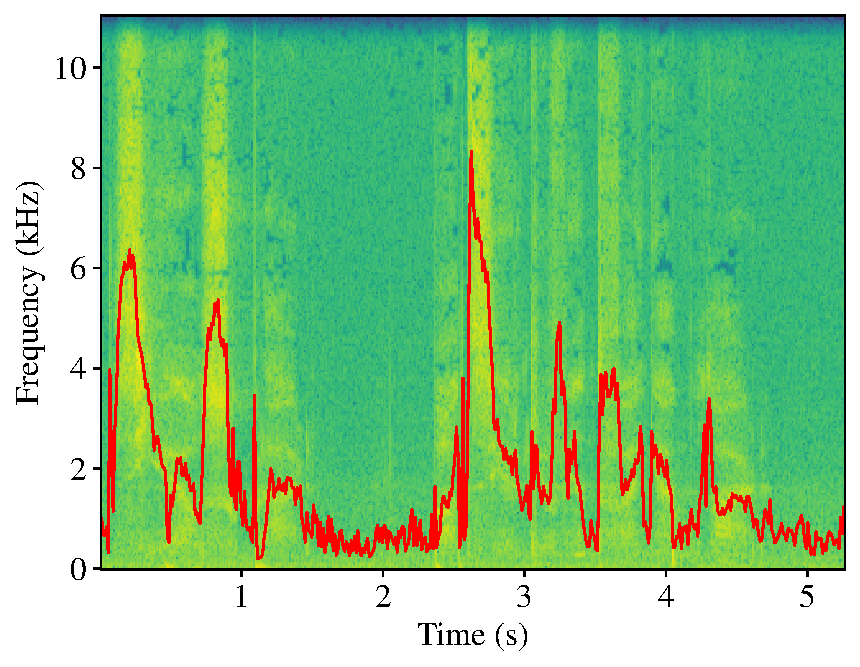
\includegraphics[width = 0.7\textwidth]{chapter6/centreOfGravity.pdf}
    \caption{\centering Spectral centre of gravity for a whispered signal - \\ {\it "Se eu soprar pode ser que o vento venha a mudar"}}
    \label{fig:centreOfGravity}
\end{figure}

\subsection{Feature Mapping}

Also in similar fashion to the work of Perrotin et.al. \cite{perrotinGlottalFlowSynthesis2020}, a sigmoid function was used to map the centre of gravity to a value between 0 and 1, but in this case defining the curve in respect to linear frequency. The sigmoid function is defined as shown in Equation (\ref{eq:cogmapping}), where $F_{vuv}$ and $F_{uv}$ are the two thresholds used to classify the signal as vocalic or unvoiced, and $\lambda$ is the slope of the sigmoid function at the geometric mean of these two frequencies. 

\begin{equation}
    \sigma(f) = \frac{1}{1-\exp\{-(f-\sqrt{F_{vuv}F_{uv}})/\lambda\}}
    \label{eq:cogmapping}
\end{equation}

Figure \ref{fig:sigmoid} shows the sigmoid curve for mapping the centre of gravity to a value between 0 and 1. The curve is defined such that the centre of gravity is mapped to 0 when it is below the unvoiced threshold, and to 1 when it is above the vocalic threshold. The slope of the curve is defined such that the curve is steepest at the geometric mean of the two thresholds, and it is set to 0.5 in this case. The slope of the curve at the average frequency $f_x = \sqrt{F_{vuv}F_{uv}}$ is given by the derivative of the sigmoid function at this point, as shown in the following equations:

\begin{equation}
    \frac{d}{df} \sigma(f) = \frac{\lambda e^{ -\lambda(f-f_x)} }{\left(e^{ -\lambda(f-f_x)} + 1 \right)^2} \text{,}
    \label{eq:sigmoidSlope}
\end{equation}

\begin{equation}
    \frac{d}{df} \sigma(f_x) = \frac{\lambda}{4} \text{.}
\end{equation}

\begin{figure}[H]
    \centering
    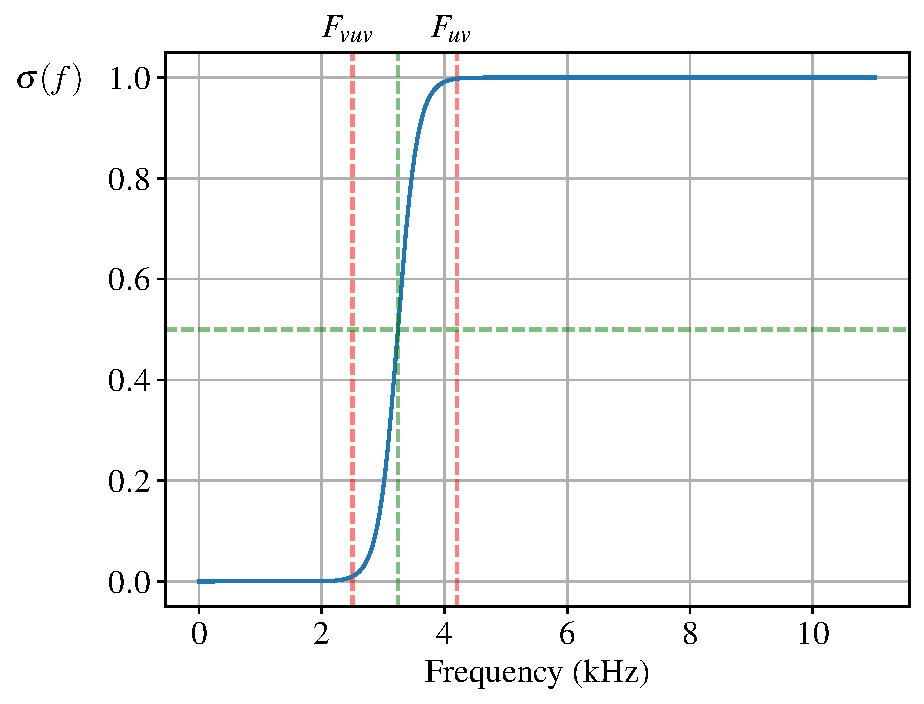
\includegraphics[width = 0.7\textwidth]{chapter6/mapping.pdf}
    \caption{Sigmoid curve for mapping the centre of gravity - $F_{vuv} = 2.5 \text{kHz}$ and $F_{uv} = 4.2 \text{kHz}$}
    \label{fig:sigmoid}
\end{figure}

The slope parameter $\lambda$ can be further parameterized in terms of the two thresholds and a new parameter $\tau$ that defines how much of space between the two points is occupied by the curve, as shown by Equation (\ref{eq:slopeParametrization}) which is adapted from \cite{perrotinGlottalFlowSynthesis2020}.

\begin{equation}
    \lambda = \frac{2}{F_{vuv}- F_{uv}} \log \left (\frac{1+\tau}{1-\tau} \right )
    \label{eq:slopeParametrization}
\end{equation}

Figure \ref{fig:mappedCoG} shows the mapped centre of gravity for the same whispered signal as in \ref{fig:centreOfGravity}, where the signal is classified as fully vocalic when the mapped value is above $F_{vuv}$, and as fully unvoiced when it is below $F_{uv}$. This is used to determine the voicing of the signal, and to trigger the $f_0(t)$ contour to be applied to the voiced segments of the signal.


\begin{figure}[H]
    \centering
    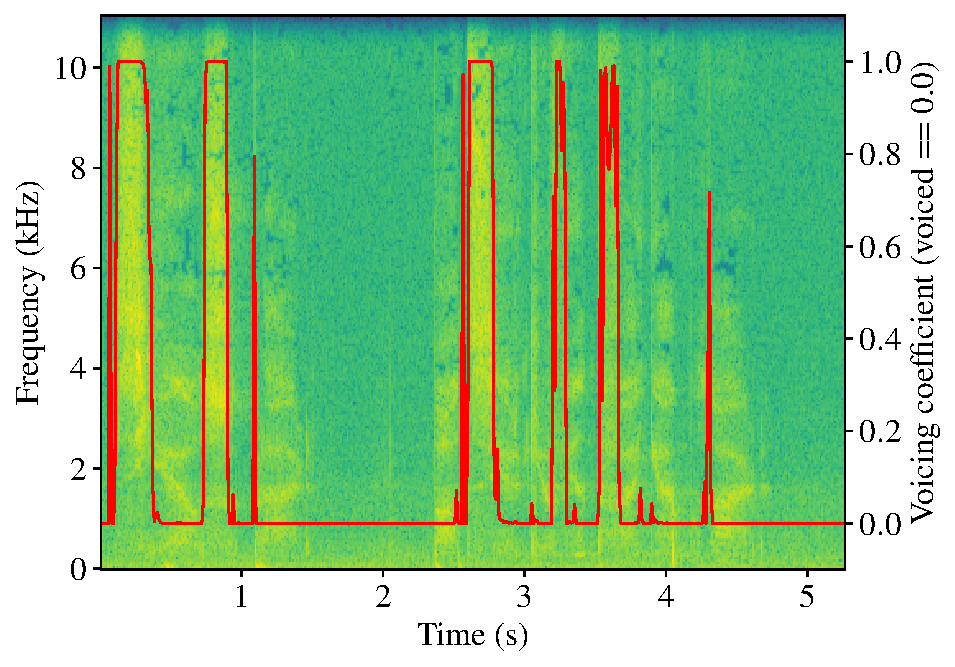
\includegraphics[width=0.7\textwidth]{chapter6/mappedCoG.pdf}
    \caption{\centering Mapped CoG for a whispered signal - {\it "Se eu soprar pode ser que o vento venha a mudar"}}
    \label{fig:mappedCoG}
\end{figure}

In reality, we actually want to always have some noise in the source excitation signal in order to avoid the presence of a purely voiced component as this can still sound unnatural. As such, in the actual system the mapping curve is scaled and shifted by a small constant factor to ensure that some level of noise is added even in purely voiced/vocalic segments. This value has been determined empirically in order to maximize the perceived naturalness of the synthesized speech.

\section{Implementation}

The first implementation of the overlap add reconstruction of voiced speech is presented in listing \ref{lst:pythonConversion}, where the system is implemented in Python for the sake of validation, as was done in the previous chapters. The results that were extracted for perceptual testing and evaluation were taken from the Python implementation, as proven in Chapters \ref{chap:pulseGen} and \ref{chap:filt}, this model has lower noise levels than the realtime physical system, and better representation of microfrequency changes to the fundamental frequency.

The system processes the input whispered speech in overlapping frames of 512 samples each. This overlap ensures continuity and smooth transitions between frames. Each input frame is windowed using the Hanning sine window, as shown in Equation (\ref{eq:windowFunc}), to reduce spectral leakage. The concatenated input frames are then subjected to the ODFT to obtain the PSD of the current frame.  In parallel, the system determines whether each frame contains voiced or unvoiced speech using the spectral centre of gravity presented previously, which gets mapped through a sigmoid function. The WAD algorithm further refines this classification by considering the energy and zero-crossing rate of the frame, ensuring that only segments with actual speech activity are processed for voicing.

Once the voiced/unvoiced decision is made, the system generates excitation signals accordingly, based on the method proposed in Figure \ref{fig:pulseGenFlow}. For voiced segments, a glottal pulse is synthesized based on the $F_0$ contour. For unvoiced segments, white noise of the same length is generated.  These excitation signals are then filtered using an LPC filter designed from the interpolated PSD of the current and previous frames. In fact, for the results presented in the next chapter, both individual pulse filtering and frame-wise filtering were used, in order to compare the impact that the smoother filter transitions have on the naturalness of the final output. %The filtered excitation signals are then added to the output buffer directly in the time domain, overlapping over top of each other. This method ensures that each frame contributes smoothly to the final output signal, maintaining continuity and naturalness. The reconstructed speech is normalized to the 16-bit PCM range to match the typical audio format used in digital systems. This step-by-step approach, combining spectral analysis, excitation generation, and LPC filtering, effectively transforms whispered speech into a more intelligible and natural-sounding voiced speech signal.

Figure \ref{fig:frameFilteringWaveform} shows the results of the individual pulse filtering and frame-wise filtering mechanisms for a given frame of whispered speech. It is to be noted that the pulse-by-pulse filtering results in a visually smoother waveform, which can be beneficial for the naturalness of the final output. The results of the perceptual testing and evaluation of the system are presented in the next chapter.

\begin{figure}[H]
    \centering
    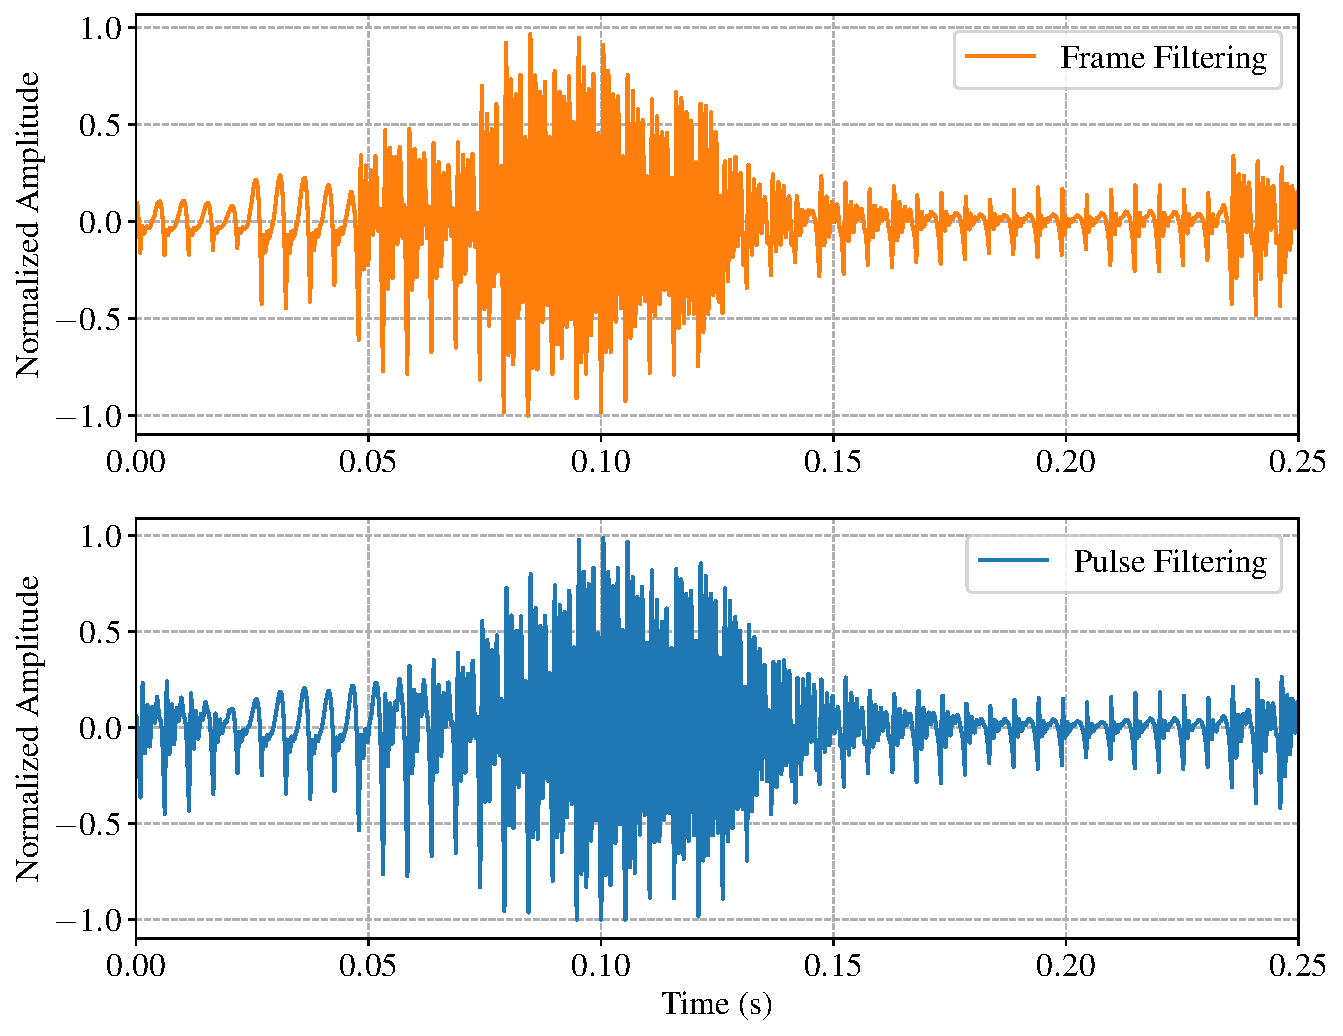
\includegraphics[width = 0.9\textwidth]{chapter6/electrolarynx.pdf}
    \caption{Frame filtered (above) and individually filtered (below) pulses}
    \label{fig:frameFilteringWaveform}
\end{figure}

Meanwhile, Figure \ref{fig:segmentedWaveform} shows the results of the whispered speech segmentation algorithm, where the unsegmented whispered speech is shown above, and the segmented whispered speech is shown below. It is to be noted that the segmentation algorithm is able to detect the voiced and unvoiced segments of the signal, which is crucial for the proper application of the $F_0$ contour and the generation of the excitation signals. The figure makes it clear that the unvoiced segments when identified are then excited by noise, and the voiced segments are excited by the glottal pulses generated by the $F_0$ contour, mixed with a lower level of noise.

\begin{figure}[H]
    \centering
    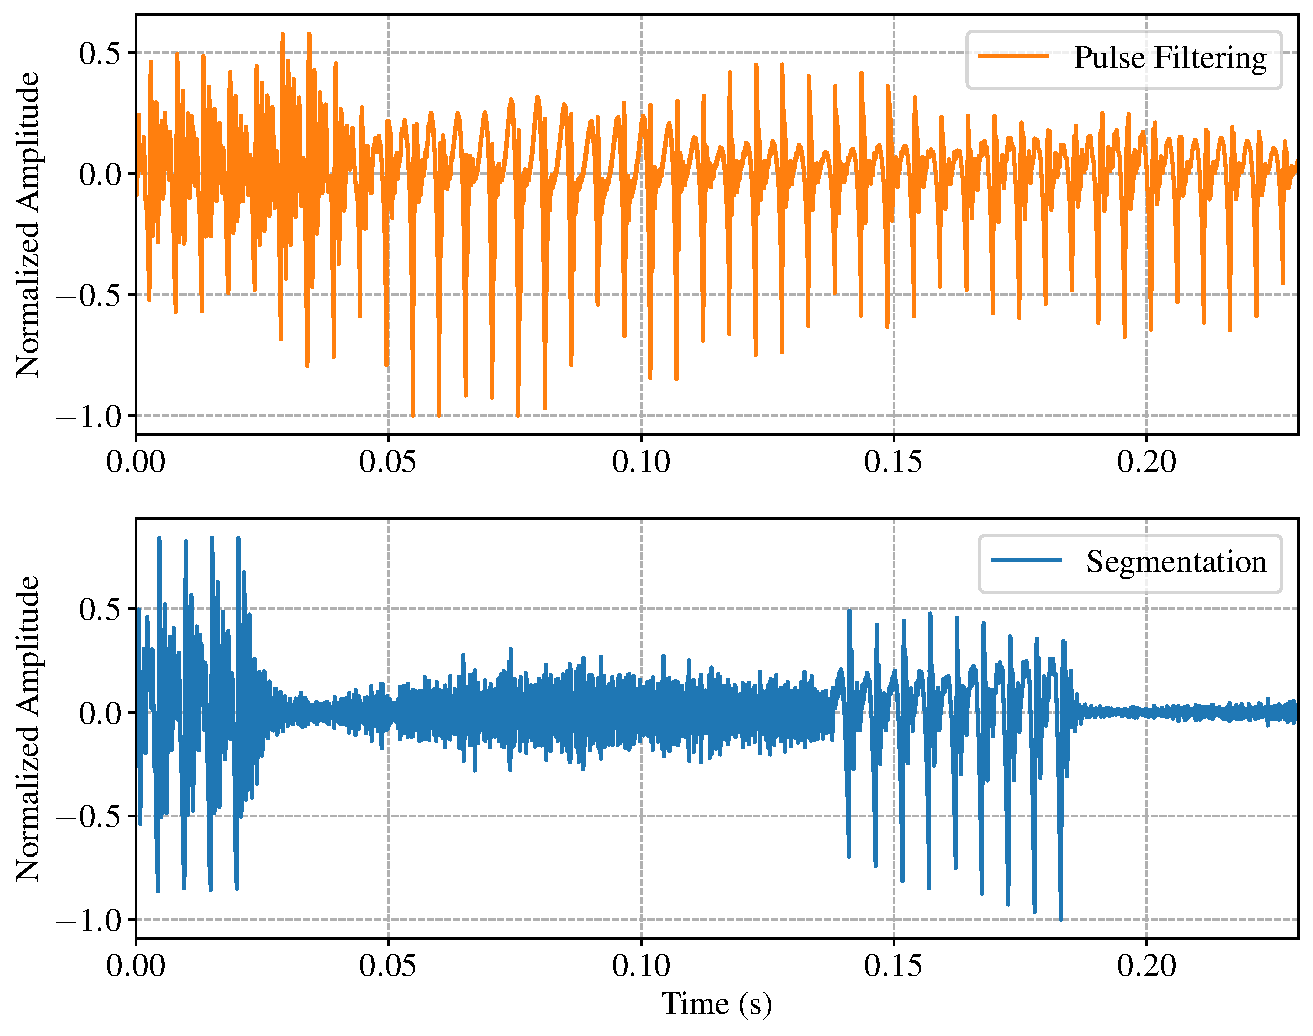
\includegraphics[width = 0.9\textwidth]{chapter6/segmentation.pdf}
    \caption{Unsegmented (above) and segmented (below) whispered speech}
    \label{fig:segmentedWaveform}
\end{figure}

%\vspace*{12mm}

\subsection{Realtime Implementation}

The system was also implemented in the STM32 environment for realtime operation. As we're using the same LPC filter as in chapter \ref{chap:filt}, the system works in the same way, with the only differences being that for each pulse the PSD is interpolated between the current and previous frames, and that the pulse is filtered in the time domain by the LPC filter. Listing \ref{lst:segmentationC} shows the implementation of the conversion algorithm in C, that was developed on top of the main function shown in listing \ref{lst:pythonConversion}.

Another relevant aspect that is worth mentioning is that of the noise signal generation. Where as in python the noise signal was generated using a normal distribution, in the STM32 environment the noise signal is generated using a simpler pseudo-random number generator. The STM32F746ng does feature the RNG peripheral, but it was decided that the use of this peripheral would be overkill for the purposes of this project, and that a much simpler Linear Congruential Generator (LCG) \cite{Iserles_1989} would suffice. The generator is implemented as shown in listing \ref{lst:noiseGenC}, and it is used to generate the noise signal that is used to excite the unvoiced segments of the signal.

\begin{lstlisting}[language=C, caption={LCG implementation in C}, label={lst:noiseGenC}]
static uint32_t seed = 1337;
#define LCG_A 1664525       // LCG multiplier
#define LCG_C 1013904223    // LCG increment
#define LCG_M 0xFFFFFFFF    // LCG modulus 2^32 - 1

/// @brief Generate a pseudo-random integer using a Linear Congruential Generator
/// @return Random integer
uint32_t randInt(){
    seed = (LCG_A * seed + LCG_C) % LCG_M;
    return seed;
}

/// @brief Generate a pseudo-random float
/// @return Random 32bit float
float32_t randFloat(){
    return 2.0f * ((float32_t) randInt() / (float32_t) LCG_M) - 1.0f;
}
\end{lstlisting}

The computation of the centre of gravity and it's mapping are also done in the STM32 environment, essentially in the same fashion as in the Python validation. As the operation is effectively a simple weighted average of the power spectrum, and the code is shown in listing \ref{lst:cogC}.

\begin{lstlisting}[language=C, caption={Centre of Gravity computation in C}, label={lst:cogC}]
/// @brief Compute the spectral centre of gravity from a frame's PSD
/// @param psd Power Spectral Density
/// @param n Total number of samples (1024)
/// @param fs Sampling Frequency
/// @return Spectral Centre of Gravity
float32_t centreOfGravity(float32_t* psd, int n, float32_t fs){
    float32_t num = 0, dem = 0;

    for (size_t i = 0; i < n / 2; i++){
        dem += psd[i];
        num += (i * fs / n) * psd[i];
    }

    return num / dem;
}

/// @brief Mapping sigmoid for computing the centre of gravity
/// @param cog Centre of gravity frequency
/// @param Fvuv Vocalic whispered threshold
/// @param Fuv Unvoiced frequency threshold
/// @param tau Sharpness coefficient (0.99)
/// @return mapped mixing coefficient
float32_t mapping(float32_t cog, float32_t Fvuv, float32_t Fuv, float32_t tau){
    float32_t k = (cog - sqrtf(Fvuv*Fuv)) * 2/(Fuv - Fvuv) * log10((1+tau)/(1-tau));    
    
    return 1/(1 + exp(-k));
}
\end{lstlisting}

One component of the system that wasn't included in the STM32 implementation shown in listing \ref{lst:segmentationC} was the whisper activity detection algorithm from previous subsections. This is due to the high computational demand of determining the zero crossing rate and energy of the signal for each frame, which made the audio produced by the STM32 stutter and fail to run in realtime. As such, the system was run in a continuous voiced mode, without the $F_0$ contour that had been established previously, which lead to some loss in perceived prosody. Despite this, the code for the whisper activity detection method is shown in listing \ref{lst:wadC}.

Due to time constraints and the effect that the board noise has on the quality of the conversion algorithm output, the results shown in the following section were taken from the Python implementation. The STM32 implementation was used to validate the conversion algorithm and to ensure that the system could run in real-time, but the results were not used for the perceptual testing and evaluation.